\documentclass[a4paper]{article}
\usepackage{fullpage, titling, amsmath, footnote, listings, graphicx}
\makesavenoteenv{tabular}
\setlength{\droptitle}{-50pt}

\title{Machine Learning Assignment 2: Decision Trees}
\author{Chris Bates, Joe Slade, Andrew West, Thomas Wood}

\begin{document}
\maketitle

\begin{itemize}
  \item The acquired decision trees, trained on the whole available dataset (6
    in total, for 6 different emotions)

    \begin{figure}[h]
      \centering
      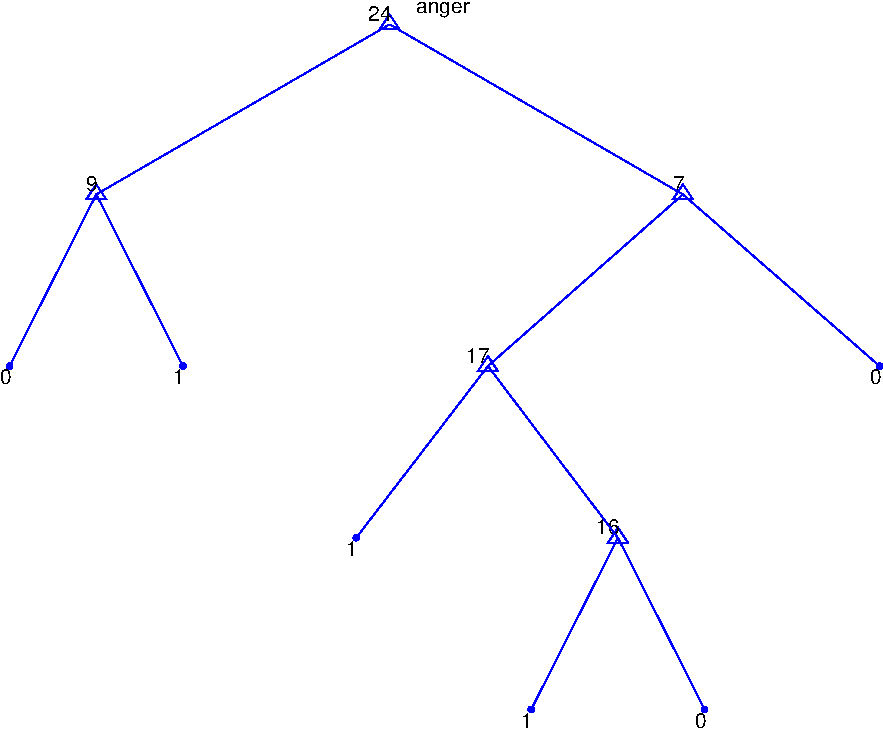
\includegraphics[scale=0.5]{graph-anger}
      \caption{Tree trained over full data set for the anger emotion}
    \end{figure}
    \begin{figure}[h]
      \centering
      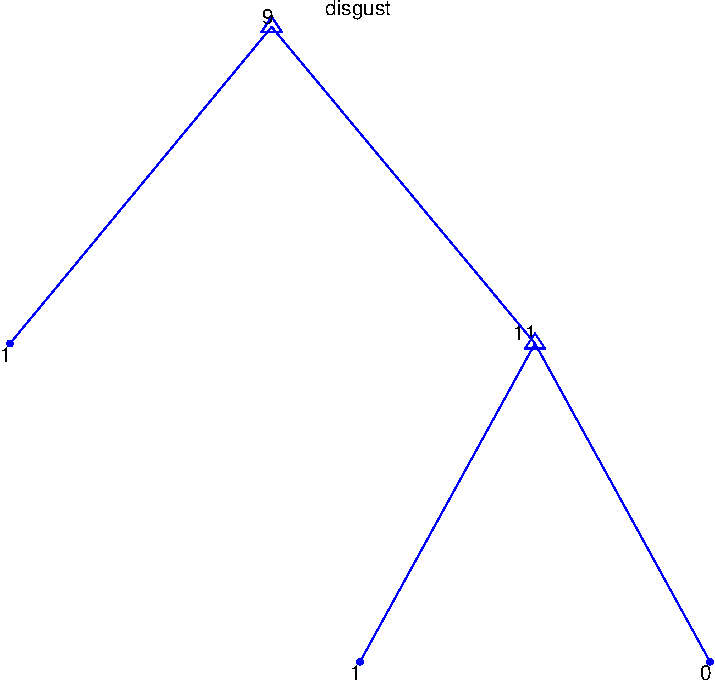
\includegraphics[scale=0.5]{graph-disgust}
      \caption{Tree trained over full data set for the disgust emotion}
    \end{figure}
    \begin{figure}[h]
      \centering
      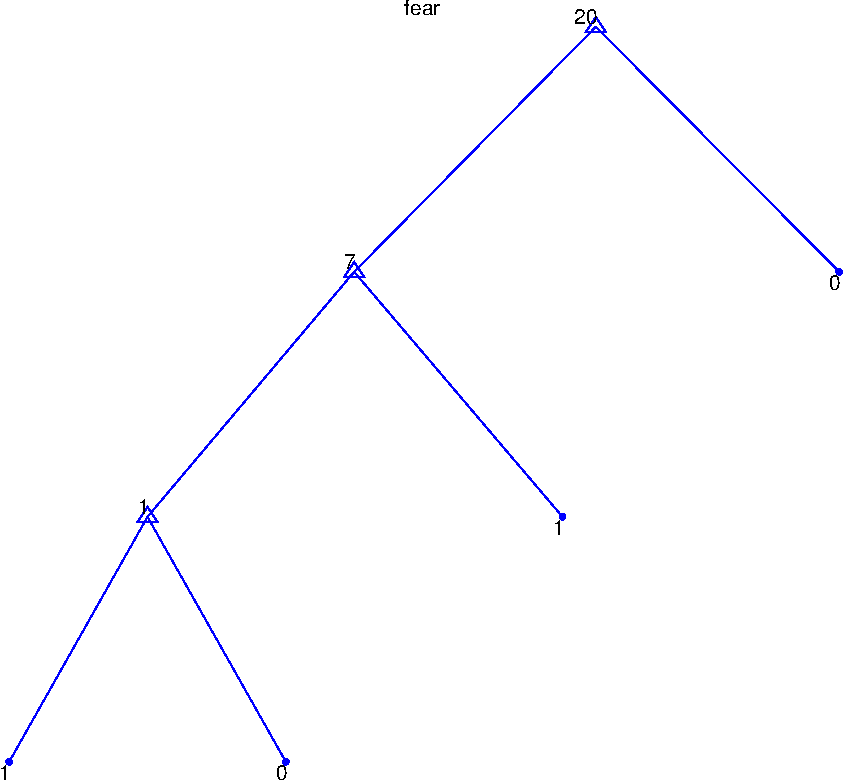
\includegraphics[scale=0.5]{graph-fear}
      \caption{Tree trained over full data set for the fear emotion}
    \end{figure}
    \begin{figure}[h]
      \centering
      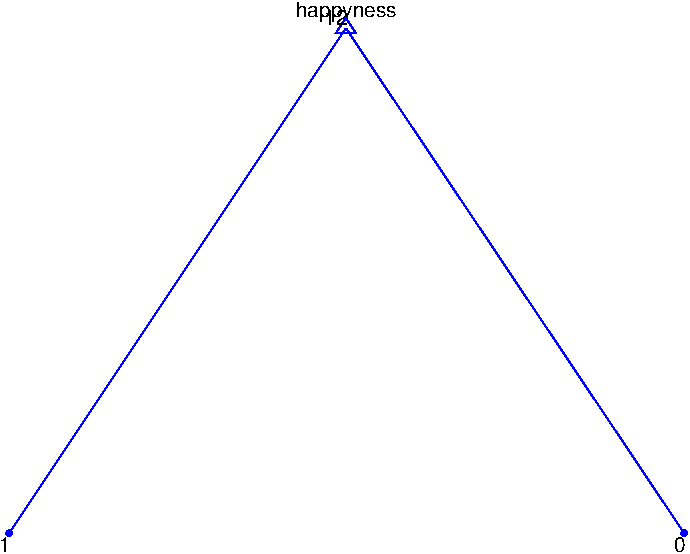
\includegraphics[scale=0.5]{graph-happyness}
      \caption{Tree trained over full data set for the happyness emotion}
    \end{figure}
    \begin{figure}[h]
      \centering
      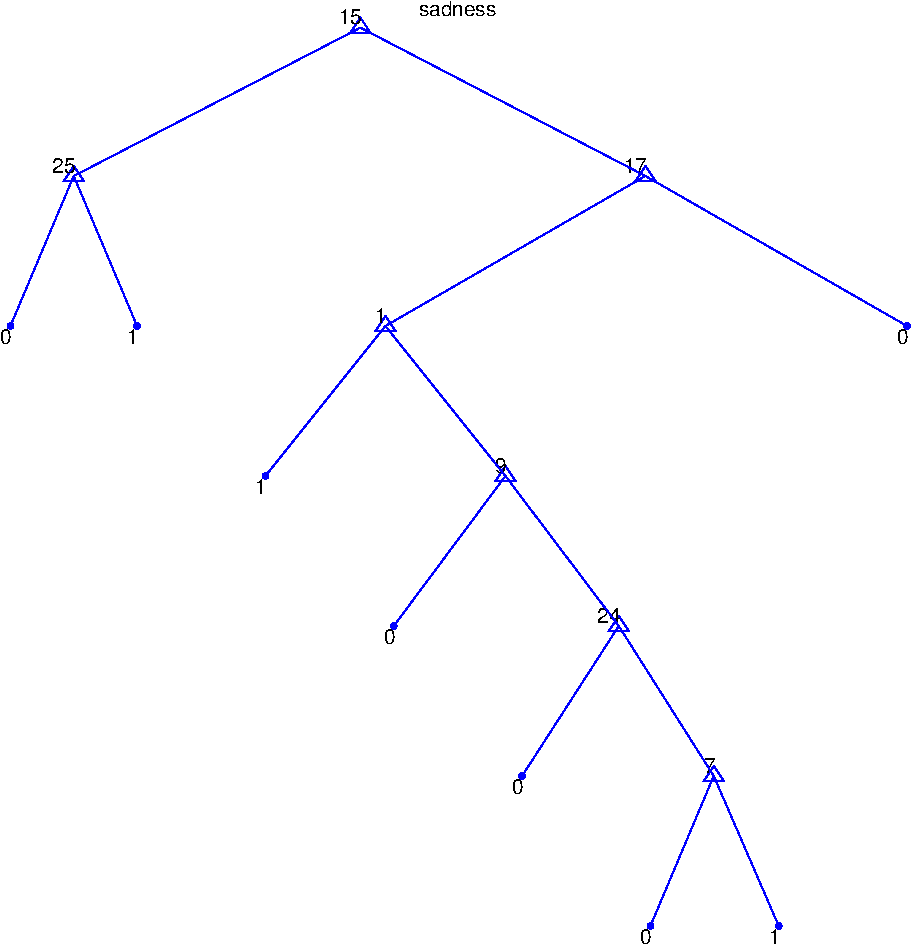
\includegraphics[scale=0.5]{graph-sadness}
      \caption{Tree trained over full data set for the sadness emotion}
    \end{figure}
    \begin{figure}[h]
      \centering
      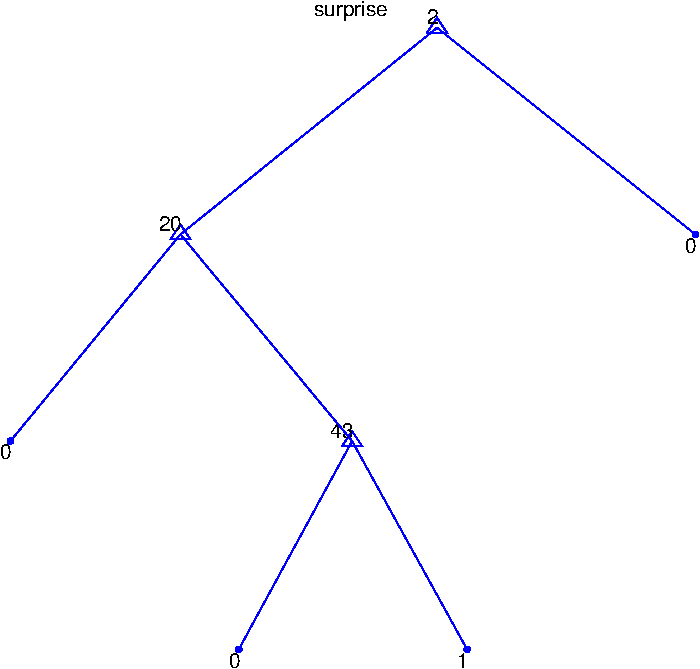
\includegraphics[scale=0.5]{graph-surprise}
      \caption{Tree trained over full data set for the surprise emotion}
    \end{figure}


  \item Each example needs to get only a single emotion assigned to it, between
    1 and 6. Explain how you made sure this is always the case in your decision
    tree algorithm.

  \item Have you encountered any ambiguity when attempting to classify a given
    sample, if yes, what strategies did you use to deal with this?

  \item Average cross validation classification results, that include:
    \begin{itemize}
      \item Confusion matrix

        \begin{tabular}{c|cccccc}
          & Anger & Disgust & Fear & Happiness & Sadness & Surprise \\
          \hline
          Anger & 10 & 0 & 1 & 0 & 1 & 0 \\
        Disgust & 1 & 21 & 0 & 0 & 0 & 0 \\
           Fear & 2 & 0 & 5 & 0 & 0 & 0 \\
      Happiness & 0 & 0 & 0 & 24 & 0 & 0 \\
        Sadness & 2 & 0 & 0 & 0 & 10 & 0 \\
       Surprise & 0 & 0 & 0 & 0 & 0 & 23 \\
        \end{tabular}

      \item Average recall, precision rates and $F_1$ value per class

        \begin{tabular}{c|cccc|ccc}
          Emotion & TP & TN & FP & FN & Precision & Recall & $F_1$ \\
          \hline
          Anger & 10 & 83 & 5 & 2 & 0.833 & 0.667 & 0.741 \\
          Disgust & 21 & 78 & 0 & 1 & 0.955 & 1.000 & 0.977 \\
          Fear & 5 & 92 & 1 & 2 & 0.714 & 0.833 & 0.769 \\
          Happiness & 24 & 76 & 0 & 0 & 1.000 & 1.000 & 1.000 \\
          Sadness & 10 & 87 & 1 & 2 & 0.833 & 0.909 & 0.870 \\
          Surprise & 23 & 77 & 0 & 0 & 1.000 & 1.000 & 1.000 \\
        \end{tabular}
      \end{itemize}

    \item \emph{Pruning is an important issue in trees. Run the prune\_example
        function, which is provided, and briefly explain how it works. It uses the
        MATLAB built-in functions for trees. Two figures should be generated showing
        two different curves. Include those figures in your report and explain why
        each curve has this shape. What is the difference between them?}

      The prune\_example function takes a set of AUs and the labels for that data,
      and builds a decision tree using MATLAB's built in functionality to build a
      decision tree from the data.

      Two graphs are produced: one from 10-cross fold-validation and one from
      resubtitution. The two graphs have equal roughly equal values for the first
      three data points. However, the 10-cross fold-validation graph has higher
      values for the next nine results than the resubtitution graph does.
      From the MATLAB documentation, the resubtitution method tends to underestimate
      the cost because it tests using the same data that the tree learned with.

      This makes sense as the tree is, in part, over-trained, and so will be likely to
      underestimate the cost of new data.


  \end{itemize}

  \end{document}


